\begin{frame}{Results: Loss Variance Analysis}

\begin{columns}[c]
\begin{column}{0.48\textwidth}
    \begin{block}{Loss Variance Comparison}
    \begin{itemize}
        \item Our method: \textbf{$<$ 0.4}
        \item Hybrid FP8: Spikes \textbf{$\geq$ 0.8}
        \item \textcolor{blue}{\textbf{50\% lower variance}}
    \end{itemize}
    \end{block}

    \vspace{0.3cm}

    \begin{alertblock}{Why More Stable?}
    \begin{itemize}
        \item E5M2 for Q/K paths
        \item Prevents overflow/underflow
        \item E4M3 for MLP stability
        \item Component-aware design
    \end{itemize}
    \end{alertblock}
\end{column}

\begin{column}{0.50\textwidth}
    \centering
    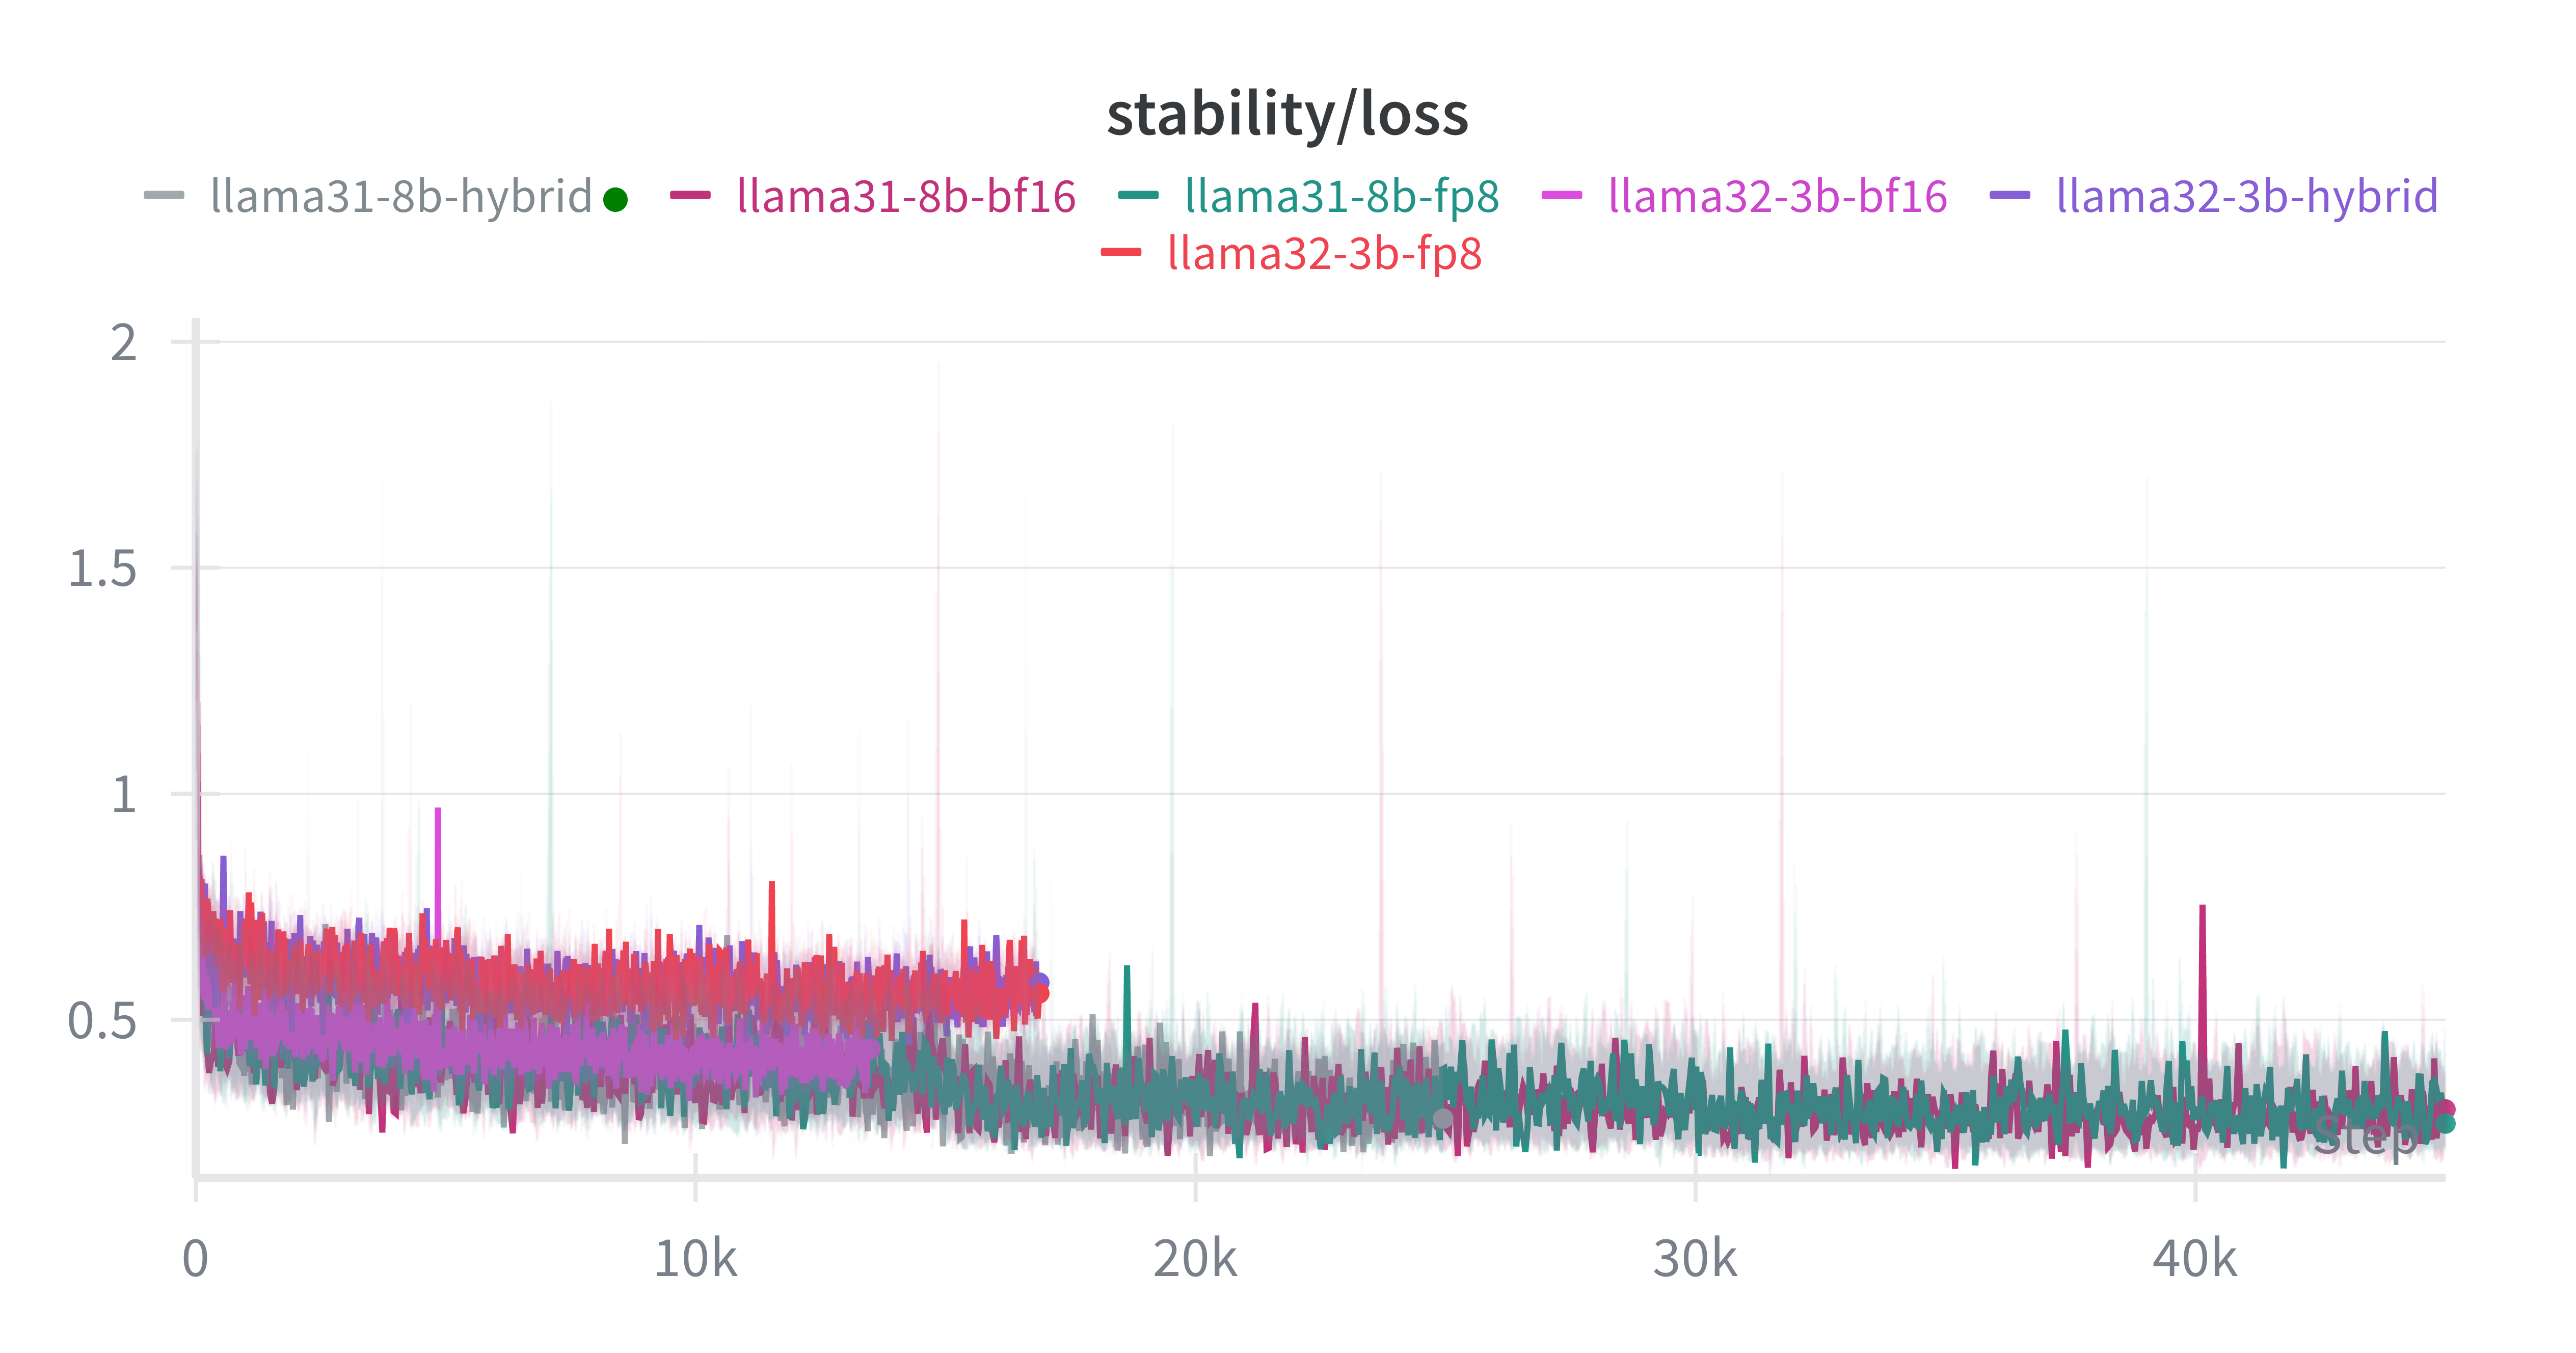
\includegraphics[width=\textwidth]{figures/numeric_stability.png}

    \vspace{0.3cm}

    \small
    \textbf{Key Observation:} Layer-wise FP8 maintains consistent low variance throughout training, while Hybrid FP8 shows periodic instability spikes.
\end{column}
\end{columns}

\end{frame}
